\chapter{Methodology of processing}
\label{methodology}
The previous chapters provided an introduction into the systems, data and methods which will be used to determine if jams characteristics, detected in \acrshort{fcd} and incident characteristics from accidents (\acrshort{baysis}) and roadworks (\acrshort{arbis}) are statistically related to each other. The research question to be answered stands as follows:

\begin{center}
	\textit{Do congestion- and incident-characteristics correlate?}
\end{center}

\medskip

The methodology to answer these research questions, will be elaborated in this chapter, starting with the detection of jams in the FCD. This also contains the generation of congestion characteristics and collection of adjacent incident. The \acrshort{fcd} is a continuous time series of datapoint which represents the mean absolute and relative speed of the street section at each 3-minute interval on a road section. In \ref{dataset_fcd} we determined that thought a manual visual analysis jams can be easily identified. This manual identification will be automated because of the amount of data representing a complete year and all Bavarian highways. The gathered tuples of congestion and incident are then processed and exported into a unified data-structure. 

The \gls{evaltool} from the \gls{congstats} service, the project which inspired this thesis, was developed for this purpose and will be expanded with required features. Afterward the stored dataset of congestion and incidents events will be analyzed for correlations and other statistic indicators.

\bigskip

\section{Detection Algorithm}
\label{methodology_detection}
First step is the detection of congestion events. The definition in \ref{definition_congestion} states that a congestion is a dense, timely and spatial accumulation of jammed cells, also describable as cluster of jammed cells. Therefore a clustering algorithm would be suitable to identify congestion events.

For the classification of the congestion events into different types, by theirs spatial and timely extends a shaping algorithm is needed. It is supposed to convert the accumulation of cells into a simple describable shape, which can be put into groups.

\subsection{Clustering of Floating-Car-Data}
\label{methodology_detection_clustering}
The term clustering is the short form of a data mining technique also called numerical taxonomy or cluster analysis with the goal of finding data structures or associations. For this purpose a multitude of algorithms where developed over time, varying in they strategies, methods and performance \parencite{Busch2004}. For example k-means or k-metoid (point distance), affinity propagation (graph distance), mean-shift (point distance), DBSCAN (nearest point distance), gaussian mixtures (mahalanobis distance to centers) or spectral clustering (graph distance), which can be sorted into the categories of partition-based, hierarchical-based and density-based clustering \parencite{Chauhan2020,Yildirim2020}.

% https://texample.net/tikz/examples/probability-tree/
% https://webis.de/downloads/theses/papers/busch_2005.pdf 1.6
%\begin{tikzpicture}[grow=right, sloped]
%\node[bag] {Cluster Algorithms}
%    child {
%        node[bag] {hierarchic}        
%             child {
%                node[end, label=right:
%                    {single-linkage, group-average}] {}                
%                edge from parent
%            }         
%            edge from parent 
%    }
%    child {
%        node[bag] {iterative}        
%            child {
%                node[end, label=right:
%                    {k-means, k-metoid, Kerninghan-Lin}] {}                
%                edge from parent
%            }         
%            edge from parent 
%    }
%    child {
%        node[bag] {density-based}        
%            child {
%                node[end, label=right:
%                    {DBSCAN, MajorClust}] {}                
%             	edge from parent
%            }
%            edge from parent
%    }
%	child {
%        node[bag] {meta-search}        
%                 child {
%                node[end, label=right:
%                    {genetic algorithms}] {}
%                edge from parent
%            }            
%            edge from parent
%    }
%    child {
%        node[bag] {statistical}        
%        child {
%                node[end, label=right:
%                    {gaussian mixtures}] {}
%                edge from parent
%            }
%            edge from parent         
%    };
%\end{tikzpicture}

\bigskip

\begin{figure}[ht]
	\centering
	\includegraphics[scale=0.5]{images/cluster_seperate.png}
	\caption{Example clustered by k-means algorithm \parencite{Yildirim2020}}
	\label{cluster_kmeans}
\end{figure}

To illustrate which problems can occur when using cluster algorithms and to defined the features which makes algorithm suitable, the k-means is used as base comparison. The figure \ref{cluster_kmeans} shows three differently colored groups of points, which are clustered into three clusters, represented by the circles around the groups. It demonstrates the general principle of clustering and was done by the common k-means algorithm with the $a$ $priori$ parameter of three clusters. 

\begin{figure}[ht]
	\centering
	\includegraphics[scale=0.4]{images/cluster_1.png}
	\includegraphics[scale=0.4]{images/cluster_2.png}
	\includegraphics[scale=0.4]{images/cluster_3.png}
	\caption{Example clustered by density-based algorithm \parencite{Yildirim2020}}
	\label{cluster_dbscan}
\end{figure}

This works well as long as the groups don't overlay, intersect or have arbitrary shapes like in the figures \ref{cluster_dbscan}. When this is the case, the k-mean may cluster loosely related point together, which actually are more strongly related to other points, because it considers every point as possible neighbor. Since jams in FCD data can overlay and have any number of shape, as suitable algorithms need to be able to handle such data.

Another issue with many clustering algorithms is the increasing runtime when processing larger amounts of data. The objective function \ref{formula_kmeans} of the exemplary k-mean states that $n$ distances are calculated for $k$ points \parencite{Santhanam2010}. With the assumption that every distance for every point will be calculated and therefore $k=n$, the Big $\Theta$ notation, commonly known as Big $O$, describing the scaleable time complexity of an algorithm, is $O(n \cdot K \cdot I \cdot d)$ ($n$ = number of points, $K$ = number of clusters, $I$ = number of iterations, $d$ = number of attributes) \parencite{Dalatu2016}. It is commonly simplified in literature to $O(n^2)$, a quadratic complexity \parencite{Pakhira2014}. The assumption also entails that in a worst case scenario $n^2$ calculations have to be computed over all iterations.

\begin{equation}
\label{formula_kmeans}
	k_{mean} =  \sum_{j=1}^k{\sum_{i=1}^n{\abs{x_i^j-c_j}}}
\end{equation}

\bigskip

A Big $O$ notation of $O(n^2)$ can generally be described as inefficient, but if we would apply the worst case scenario as an example on the data of the highway A3 and a timeframe of 24 hours, which contains 836.752 data points, the runtime issue becomes quite obvious. As the equation \ref{equation_kmeans_nn} show, the total number of calculation is quite high, resulting in a considerable runtime. \parencite{Busch2004}

\begin{equation}
\label{equation_kmeans_nn}
	 = 836752 \cdot 836752 = 700.153.909.504 = 7 \cdot 10^{11}
\end{equation}

\bigskip

Entering density-based methods, which are better suited to identify distinctive, arbitrary clusters in, by looking for a contiguous region of high point density, separated from others by contiguous regions of low point density \parencite{Chauhan2020}. These do not necessarily have less runtime, but better cluster representation.

\subsubsection{Density Clustering Algorithm}
The DBSCAN algorithm, standing for \textbf{d}ensity-\textbf{b}ased \textbf{s}patial \textbf{c}lustering of \textbf{a}pplications with \textbf{n}oise, is able to find arbitrary shaped cluster and clusters by considering the spatial density, which also represents noise. The basic idea of this algorithm is to form cluster of points, which are close too \textbf{many} other points of the cluster. For this strategy two thresholds parameters are needed. The first being the minimal size of a cluster, referred to as $MinPts$, which defines the minimum number of points necessary to form a cluster. And secondly the maximum distance threshold between points, $eps$ ($\varepsilon$), to be considered as neighbors and become part of a cluster. These thresholds classify a data point as core point, (directly) density-reachable point or noise. \parencite{Yildirim2020,Chauhan2020,Padro2017}

\begin{itemize}
	\item A \textbf{core} point $q$ has at least $MinPts$ points around them within the neighborhood $\varepsilon$, including itself.
    \item \textbf{Directly density-reachable} border points have at least one core point within the neighborhood $\varepsilon$.
     \item \textbf{Density-reachable} border points have at least one core point within the neighborhood $\varepsilon$ of a cain of points $p_1,p_2,...p_n$.
 	\item \textbf{Noise} or outliner point are neither core points nor are they density-reachable and therefore have less than $MinPts$ in their neighborhood $\varepsilon$, including itself.
\end{itemize}

The general procedure of the algorithm is as follows \parencite{Zhao2018}, with the input of $n$ points, neighborhood radius $\varepsilon$ and density threshold $MinPts$:

\begin{itemize}
	\item[\textbf{1.}] Mark all points as \textit{unvisited}
	\item[\textbf{2.}] Choose point $p$ randomly from all \textit{unvisited} points.
	\begin{itemize}
		\item[\textbf{a.}] Choose point $p$ randomly from all \textit{unvisited} points and mark $p$ as \textit{visited}.
		\item[\textbf{b.}] Count points in the neighborhood $\varepsilon$ to check if $p$ is core point. If $p$ is core point, create new cluster $C$ and add all directly density-reachable and \textit{unvisited} points. Otherwise mark $p$ as noise.
		\item[\textbf{c.}] Choose point $p'$ randomly from all \textit{unvisited} points of $C$ and mark $p$ as \textit{visited}.
		\item[\textbf{d.}] Count points in the neighborhood $\varepsilon$ to check if $p'$ is core point. If $p$ is core point add all directly density-reachable points, which do not already belong to a cluster, to $C$. Otherwise mark $p$ as noise.
		\item[\textbf{e.}] Repeat \textbf{c} and \textbf{d} until there are no \textit{unvisited} points left in $C$.	
	\end{itemize} 
	\item[\textbf{3.}] Repeat \textbf{2} until all points are \textit{visited} 
\end{itemize}

%https://www.kde.cs.uni-kassel.de/wp-content/uploads/ws/LLWA03/fgml/final/Kirchner.pdf
%https://www.researchgate.net/publication/322729622_Characterizing_Diffusion_Dynamics_of_Disease_Clustering_A_Modified_Space-Time_DBSCAN_MST-DBSCAN_Algorithm
%https://www.nature.com/articles/s41598-017-12852-z
%http://citeseerx.ist.psu.edu/viewdoc/download?doi=10.1.1.63.1629&rep=rep1&type=pdf
%http://cucis.eecs.northwestern.edu/publications/pdf/HAL18.pdf

\subsubsection{Artificial Distance Measuring}
The algorithm is based on the density of points. This density representation is achieved via checking the neighborhood $\varepsilon$ against calculation of distance from point $A$ to $B$, typical the Euclidean distance, which is based on the pythagorean theorem (see equation \ref{formula_euclidean} \parencite{Erhard2020}).

\begin{figure}[ht]
	\centering
	\begin{tikzpicture}[scale=0.7]
			
		\draw [<->,thick] (0,5) node (yaxis) [above] {$y$}
	        |- (10,0) node (xaxis) [right] {$x$};
	        
	    \foreach \x in {1,...,9}
	    	\draw[black!30] (\x,0) -- (\x,5);
	    	
	   	\foreach \y in {1,...,4}
	    	\draw[black!30] (0,\y) -- (10,\y); 
	        
	    \foreach \x in {1,...,9}
	    	\draw (\x,1pt) -- (\x,-3pt)
			node[anchor=north] {\x};
			
		\foreach \y in {1,...,4}
	    	\draw (1pt,\y) -- (-3pt,\y) 
	     	node[anchor=east] {\y}; 
	
		\coordinate[label={270:$ $}] (C) at (8,1);
		\coordinate[label={180:$A$}] (A) at (2,1);
		\coordinate[label={30:$B$}] (B) at (8,4);
	
		\draw (C) -- (A)node[midway,below left]{$a$} -- (B)  -- cycle node[midway,below right]{$b$};
	       
		\draw [dashed] (C) -- ($(A)!(C)!(B)$) coordinate (P) node [midway, left]{$h$};
		
		\draw[decorate,decoration={brace,raise=12pt,amplitude=5pt}] (A) -- (B);
		
		\path (B) -- (P) node[midway,above]{$$} -- (A) node[midway,above]{$$} ($($(A)!0.5!(B)$)!1.2cm!90:(B)$) node {$d_{A,B}$}; % You can nest calc syntax!
		
		\filldraw[fill=white] (C) -- ($(C)!2mm!(A)$) coordinate (U) -- ($(U)!2mm!90:(C)$) 
	      --($(C)!2mm!(B)$) --cycle;
		
		\draw ($(P)!2mm!(C)$) coordinate (V) -- ($(V)!2mm!90:(C)$) --($(P)!2mm!(B)$);

	\end{tikzpicture}
	\caption{Euclidian distance in 2-dimensional euclidian space}
\end{figure}

\begin{equation}
	d_{A,B} = \sqrt{a^2 + b^2} = \sqrt{(x_B-x_A)^2+(y_B-y_A)^2}
	\label{formula_euclidean}
\end{equation}

\medskip

As shown above, the euclidean distance calculation assumes a Euclidean space, meaning equal scaling of both axis, which is not the case with FCD. The 2D-space of the FCD is defined by a spatial and a temporal dimension, which are scaled differently as mentioned in section \ref{dataset_fcd}. The vertical axis shows the temporal dimension is regular scales in 3 minute intervals. The horizontal axis is the spatial extend, scaled in one cell per step, representing one road link (road link are rather small subsection of roads, defining the course), which vary heavily in their length. This can be visualized like:

\begin{figure}[ht]
	\centering	
	\begin{tikzpicture}[scale=0.7]	
	
		\draw [<->,thick] (0,5) node (yaxis) [above] {$y$}
	        |- (10,0) node (xaxis) [right] {$x$};
	    % X Axis lines  
	    \draw[red] (0.7,1pt) -- (0.7,-3pt)
		node[anchor=north] {70}; 
	    \draw[red] (1.5,1pt) -- (1.5,-3pt)
		node[anchor=north] {110};   
	    \draw[red] (2.5,1pt) -- (2.5,-3pt)
		node[anchor=north] {250};
		\draw[red] (4,1pt) -- (4,-3pt)
		node[anchor=north] {400};
		\draw[red] (7,1pt) -- (7,-3pt)
		node[anchor=north] {700};
		\draw[red] (8.3,1pt) -- (8.3,-3pt)
		node[anchor=north] {830};
		\draw[red] (9.3,1pt) -- (9.3,-3pt)
		node[anchor=north] {930};
	    \foreach \x in {0.7,1.5,2.5,4,7,8.3,9.3}
	    	\draw[black!30] (\x,0.1) -- (\x,4.9);
	    % Y Axis lines	
		\draw[red] (1pt,1) -- (-3pt,1) 
	     	node[anchor=east] {3}; 
	    \draw[red] (1pt,2) -- (-3pt,2) 
	     	node[anchor=east] {6}; 
	    \draw[red] (1pt,3) -- (-3pt,3) 
	     	node[anchor=east] {9}; 
	    \draw[red] (1pt,4) -- (-3pt,4) 
	     	node[anchor=east] {12}; 
	    \foreach \y in {1,...,4}
	    	\draw[black!30] (0.1,\y) -- (9.9,\y); 
	    	
	    \coordinate[label={270:$ $}] (C) at (7,1);
		\coordinate[label={180:$A$}] (A) at (1.5,1);
		\coordinate[label={30:$B$}] (B) at (7,4);
	
		\draw (C) -- (A)node[midway,below left]{$a$} -- (B)  -- cycle node[midway,below right]{$b$};
	       
		\draw [dashed] (C) -- ($(A)!(C)!(B)$) coordinate (P) node [midway, left]{$h$};
		
		\draw[decorate,decoration={brace,raise=12pt,amplitude=5pt}] (A) -- (B);
		
		\path (B) -- (P) node[midway,above]{$$}-- (A) node[midway,above]{$$} ($($(A)!0.5!(B)$)!1.2cm!90:(B)$) node {$d_{A,B}$}; % You can nest calc syntax!
		
		\filldraw[fill=white] (C) -- ($(C)!2mm!(A)$) coordinate (U) -- ($(U)!2mm!90:(C)$) 
	      --($(C)!2mm!(B)$) --cycle;
		
		\draw ($(P)!2mm!(C)$) coordinate (V) -- ($(V)!2mm!90:(C)$) --($(P)!2mm!(B)$);
				
	\end{tikzpicture}
	\caption{Euclidian distance in 2-dimensional non-euclidian space}
\end{figure}

\bigskip

This makes a direct application of the Euclidian distance invalid to calculate the distance from point $A$ to point $B$. But then how can distances be represented in this 2D-space with different units? The solution developed for this application is to expand the 2D-representation of time and space into a 3D-representation of time, space and speed (absolute mean traveling speed is part of \acrshort{fcd}, see section \ref{dataset_fcd}). Because speed $[km/h]$ consist of both time $[min]$ and space $[m]$ is allows for the introduction of the common unit travel time, which can be comprise from these three parameters traveling speed, time duration and link length. At this point it has to be noted, the implemented definition does not represent actual travel time but server the need of being common unit and rough representation. To separate both terms the term \textit{artificial travel time} will be used instead of \textit{travel time}.

\begin{figure}[ht]
	\centering	
	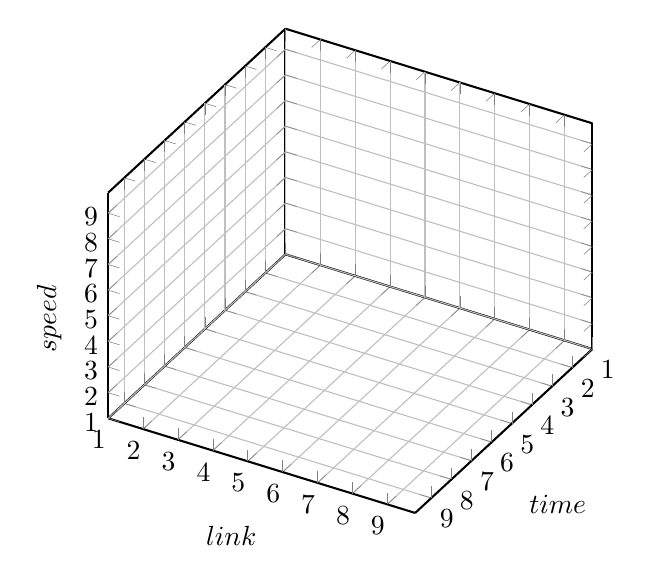
\begin{tikzpicture}
	
		\begin{axis}[
			view={120}{40},
			width=220pt,
			height=220pt,
			grid=major,
			z buffer=sort,
			xmin=1,xmax=9,
			ymin=1,ymax=9,
			zmin=1,zmax=9,
			enlargelimits=upper,
			xtick={1,...,9},
			ytick={1,...,9},
			ztick={1,...,9},
			xlabel={$time$},
			ylabel={$link$},
			zlabel={$speed$},
			point meta={x+y+z+3},
			colormap={summap}{
				color=(black); color=(blue); 
				color=(black); color=(white) 
				color=(orange) color=(violet) 
				color=(red)
			},
			scatter/use mapped color={
				draw=mapped color,fill=mapped color!70},
			]
			% http://pgfplots.sourceforge.net/gallery.html. 
		\end{axis}
		
	\end{tikzpicture}
	\caption{3-dimensional space representation of \acrshort{fcd}}
\end{figure}

Assuming an 3D-space of $time steps$ $\equiv x=[x_1,...,x_n]$ , $space$ $\equiv y=[y_1,...,y_n]$ and $speed$ $\equiv z=[z_1,...,z_n]$ the mathematical definition of calculation for the distance from point $A$ to point $B$ is as follows.

\paragraph{Time dimension} Traveling just in the time dimension is not actual possible, hence the term artificial travel time. But assuming that both point $A$ and $B$ are at the same \textbf{space} step, the distance is calculated by:
\begin{equation}
	t_{x,A,B}^{artificial} = (x_B - x_A) \cdot ( x_{interval} + 1 )
	\label{equation_t_v_time}
\end{equation}
\begin{itemize}
	\setlength\itemsep{0.1em}	
	\item[] $x_A | x_B$ is the $x$ index of point $A | B$
	\item[] $x_{interval}$ is the time interval or step duration
\end{itemize}

\begin{lstlisting}[basicstyle=\tiny, style=java, caption={vertical distance calculation}, label=lst:distance_calc_vertical] 
    /**
     * Computes the vertical distance from A to B in [s]
     *
     * @param a The indexes of from where, with [0] = stepIdx and [1] = linkIdx
     * @param b The indexes of to where, with [0] = stepIdx and [1] = linkIdx
     * @return The travel time in seconds
     */
    public double computeVertical(final int[] a, final int[] b) {
        // make sure that cells are on the same link
        assert a[1] == b[1];
        // calculate number of steps between cells
        final int deltaSteps = (Math.abs(b[0] - a[0]));
        // the vertical travel time in [s] is sum of ( time steps [idx] * step duration [min] * 60 [s] ) and therefore is inclusive
        return deltaSteps * stepDuration * 60;
    }
\end{lstlisting}

\paragraph{Space dimension} Traveling just through space is also not actual possible, but in the artificial travel time. Under the assumption that point $A$ and point $B$ are in the \textbf{time} step, the distance is calculated by:  
\begin{equation}
	t_{y,A,B}^{artificial} = (\frac{y_{A}^{length}}{2}  \cdot z_{A}^{speed}) + (\frac{y_{B}^{length}}{2} \cdot z_{B}^{speed}) + \sum_{i}^{y_A + 1,...,y_B - 1} (y_{i}^{length} \cdot z_{i}^{speed})
\end{equation}
\begin{itemize}
	\setlength\itemsep{0.1em}	
	\item[] $y_A | y_B$ is the $y$ index of point $A | B$
	\item[] $y_{length}$ is the length of the link
	\item[] $z_{speed}$ is the speed in the cell
\end{itemize}

\begin{lstlisting}[basicstyle=\tiny, style=java, caption={horizontal distance calculation}, label=lst:distance_calc_horizontal] 
	/**
	* Computes the horizontal distance from A to B in [s]
	*
	* @param a_idx The indexes of from where, with [0] = stepIdx and [1] = linkIdx
	* @param b_idx The indexes of to where, with [0] = stepIdx and [1] = linkIdx
	* @return The travel time in seconds
	*/
   public double computeHorizontal(final int[] a_idx, final int[] b_idx) {
	   // make sure that cells are in the same time step
	   assert a_idx[0] == b_idx[0];
	   final int stepIdx = a_idx[0];
	   // space travel time in [s] is sum of ( link length [m] / ( the speed [km/h] * 1000 / 3600 ) [m/s] )
	   double spaceTime = 0;
	   int lowerLinkIdx = Math.min(a_idx[1], b_idx[1]);
	   int upperLinkIdx = Math.max(a_idx[1], b_idx[1]);
	   for (int i = lowerLinkIdx + 1; i < upperLinkIdx; i++) {
		   double travelSpeed = speedMatrix[stepIdx][i] * 1000D / 3600;
		   spaceTime = spaceTime + (linkLengths[i] / travelSpeed);
	   }
	   // add half travel time from start and end cell (middle to middle or inclusive)
	   double travelSpeedA = speedMatrix[stepIdx][lowerLinkIdx] * 1000D / 3600;
	   spaceTime = spaceTime + (linkLengths[lowerLinkIdx] / travelSpeedA / 2);
	   double travelSpeedB = speedMatrix[b_idx[0]][upperLinkIdx] * 1000D / 3600;
	   spaceTime = spaceTime + (linkLengths[upperLinkIdx] / travelSpeedB / 2);
	   return spaceTime;
   }
\end{lstlisting}

\paragraph{Diagonal time/space dimension} The diagonal distance or time/space distance is based on the concept of the Euclidian distance. Although the conversion to the artificial travel time fixes the disparity of the axis units, a calibration for weighing the time and space axis is still necessary. This achieved by using the aimed gap thresholds to form a calibrator value, which scales the axis appropriately, to be of equal scaling. This makes it possible to use the artificial travel time a distance parameters, for horizontal, vertical and diagonal movements.
\begin{equation}
	t_{x,y,A,B}^{artificial} = \sqrt{(t_{x,A,B}^{art})^2 + (t_{y,A,B}^{art} \cdot c)^2}
\end{equation}
\begin{equation}
	v_{A,B}^{mean} = \sum_{ij}^{xy_A + 1,...,xy_B - 1} z_{ij}^{speed}
\end{equation}
\begin{equation}
	c = \frac{t_{min,gap} \cdot v_{freeflow}}{l_{min,gap}}
\end{equation}
\begin{itemize}
	\setlength\itemsep{0.1em}	
	\item[] $xy_A | xy_B$ is the $xy$ index of point $A | B$
	\item[] $z_{speed}$ is the speed in the cell
	\item[] $v^{mean}$ is mean speed in the area between $A$ and $B$
	\item[] $c$ is the time-space calibrator
	\item[] $t_{min,gap}$ is the the aimed time gap
	\item[] $l_{min,gap}$ is the the aimed space gap
	\item[] $v_{freeflow}$ is the assumed free flowing speed (typically 130\,[km/h])
\end{itemize}

\begin{lstlisting}[basicstyle=\tiny, style=java, caption={diagonal distance calculation}, label=lst:distance_calc_diagonal] 
	/**
	* Computes the distance between two n-dimensional vectors.
	* <p>
	* The vectors are not required to have the same dimension, but should represent the
	* [0] time step and [1] link step
	*
	* @param a The first vector with [0] = stepIdx and [1] = linkIdx
	* @param b The second vector with [0] = stepIdx and [1] = linkIdx
	* @return The distance between the two vectors
	* @throws DimensionMismatchException If the array lengths differ.
	*/
   public double computeDistance(int[] a, int[] b) throws DimensionMismatchException {
	   if (a.length != b.length) {
		   throw new DimensionMismatchException(a.length, b.length);
	   }
	   if (a[0] == b[0] && a[1] == b[1]) {
		   // same link and same step -> travel time from A to B is zero
		   return 0;
	   } else if (a[1] == b[1]) {
		   // same link -> travel time from A to B can be calculated vertically
		   return computeVertical(a, b);
	   } else if (a[0] == b[0]) {
		   // same step -> travel time from A to B can be calculated horizontally
		   final double minimalVerticalTravelTime = stepDuration * 60 * 0.5;
		   return Math.sqrt(Math.pow(minimalVerticalTravelTime, 2) + Math.pow(computeHorizontal(a, b) * horizontalCalibrator, 2));
	   } else {
		   // compute diagonal with pythagorus and mean of speeds
		   final int sigT = a[0] > b[0] ? -1 : 1;
		   final int sigX = a[1] > b[1] ? -1 : 1;
		   final int deltaSteps = sigT * (Math.abs(b[0] - a[0]) - 1);
		   final int deltaLinks = sigX * (Math.abs(b[1] - a[1]) - 1);
		   // collect absolute speed in rectangle from cell A and cell B
		   final int[] absoluteSpeeds = new int[(Math.abs(deltaSteps) + 2) * (Math.abs(deltaLinks) + 2)];
		   int absoluteSpeedsCounter = 0;
		   for (int i = 1; i <= Math.abs(deltaSteps) + 2; i++) {
			   for (int j = 1; j <= Math.abs(deltaLinks) + 2; j++) {
				   absoluteSpeeds[absoluteSpeedsCounter] = speedMatrix[a[0] + sigT * i - sigT][a[1] + sigX * j - sigX];
				   absoluteSpeedsCounter++;
			   }
		   }
		   // compute mean travel time over cell rectangle
		   int speedSum = 0;
		   for (int i = 0; i < absoluteSpeedsCounter; i++) {
			   speedSum += absoluteSpeeds[i];
		   }
		   final double meanSpeed = (double) speedSum / absoluteSpeedsCounter;
		   // compute the total space between the points in [m] by adding up all link lengths
		   final int deltaSpace;
		   if (deltaLinks == 0) {
			   deltaSpace = 0; // if the cell A and B are right next to each other -> no spacial distance
		   } else if (sigX < 0) {
			   int tempDeltaSpace = 0;
			   tempDeltaSpace += linkLengths[a[1]] / 2; // add beginning cell length half
			   for (int i = b[1] + 1; i < a[1]; i++) {
				   tempDeltaSpace += linkLengths[i];
			   }
			   tempDeltaSpace += linkLengths[b[1]] / 2; // add ending cell length half
			   deltaSpace = tempDeltaSpace;
		   } else {
			   int tempDeltaSpace = 0;
			   tempDeltaSpace += linkLengths[a[1]] / 2; // add beginning cell length half
			   for (int i = a[1] + 1; i < b[1]; i++) {
				   tempDeltaSpace += linkLengths[i];
			   }
			   tempDeltaSpace += linkLengths[b[1]] / 2; // add ending cell length half
			   deltaSpace = tempDeltaSpace;
		   }
		   // compute the total space time in [s] from the link lengths and absolute speeds
		   final int deltaSpaceTime;
		   deltaSpaceTime = (int) Math.round(deltaSpace / (meanSpeed * 1000 / 3600));
		   // compute the total time between the points in [s], can be done vertically
		   final double deltaTime = computeVertical(new int[]{a[0], a[1]}, new int[]{b[0], a[1]});
		   // compute and return the mean travel time from A to B
		   return Math.sqrt(Math.pow(deltaTime, 2) + Math.pow(deltaSpaceTime * horizontalCalibrator, 2));
	   }
   }
\end{lstlisting}

% TODO read and add infos: https://diglib.tugraz.at/download.php?id=576a764ebc982&location=browse \parencite{Hatbauer2011}

\subsubsection{Performance Tuning}
Leaving out the runtime implication of the distance measurer, the complexity of DBSCAN clustering algorithm can be as low as $O(nlog_n)$. This best case scenario can be achieved by using indexing system to store the clustering data in a space representation, like a 2D-Tree. This reduces the number of point to check for neighborhood, from all points in a worst case scenario (equivalent to a complexity of $O(n^2)$), to just adjacent points \parencite{Chauhan2020}. For initially testing a $kd$-Tree was implemented, which stores data points as leafs in a tree, where the nodes divide the space consecutively in the $x$ and $y$ dimension \parencite{Hucker2020,Dalitz2009}. This improved the runtime performance, but also added complexity, which endorsed the use of a natively implemented data structure, like the TreeMap. The TreeMap strictly speaking is no a 2D-Tree, but has an average complexity of $O(nlog_n)$ and be used as a 2D-Tree by filtering with two parameters (see source code ??). \parencite{Baeldung2020_1,Baeldung2020_2}

% https://de.wikipedia.org/wiki/K-d-Baum
% https://github.com/jmhodges/kdtree2/blob/master/doc/kdtree2.tex

To further accelerate the algorithm, is is implemented with support of parallel computation or threading, which allows the executing Java VM to used multiple CPU cores and run multiple processes in parallel.

\subsubsection{Calibration}
Parameter calibration and estimation is a vital task when implementing algorithms. The DBSCAN uses the neighborhood $\varepsilon$ and $minPoints$ parameters as adjustments. If $\varepsilon$ is too small, part of the data will not be clustered, since the distances to many points is below the threshold. These points are therefore considered as outliner/noise and reduce the actual size of the cluster or make the cluster neglect able because $minPoints$ will not be reached to create a dense region. On the other side, if the value is chosen too high, a high number of point will be considered as one cluster, when they should be multiple separate clusters. The $minPoints$ threshold should generally satisfy $minPoints > D + 1$ and should be high enough for our implementation to neglect small and arbitrary jams. \parencite{Padro2017}. For the implemented variation of distance measuring the aimed time gap $t_{min,gap}$ and aimed space gap $l_{min,gap}$ threshold also need to be set. This is necessary to scale the axis so that they represent the aimed thresholds through neighborhood $\varepsilon$. The following values are the result of iterative testing, to find the most representable cluster consolidation results. 

\begin{itemize}
	\item Aimed spatial gap : $l_{min,gap} = 5000 \,[m]$
	\item Aimed temporal gap : $t_{min,gap} = 6 \,[min]$
	\item Virtual travel-time gap $\varepsilon = t_{min,gap}^{artificial} = 360 \,[s]$
\end{itemize}

\subsection{Pre and Post Data Revision}
Datasets are rarely flawless and as mentioned in section \ref{dataset_fcd}, the provided FCD dataset has some defects. To reduce these defects before the clustering, static speed blocks are removed as pre-processing measure. When the speed is consistent in a a continuous time and space extent, we assume that the data block is flawed because of the implausible consistent speeds. (see source code ??) 

As post processing, clusters which are too short in duration and length are removed. We assume that below a threshold a cluster can not be considered as a jam, and should be neglected. The following values for the minimal duration and length of a congestion where used. (see source code ??)

\begin{itemize}
	\item Minimum spatial length of an congestion event : $l_{min} = 1000 \,[m]$
	\item Minimum temporal duration of an congestion event : $t_{min,gap} = 9 \,[min]$
\end{itemize}

\subsection{Shaping}
\label{methodology_detection_shaping}
For a shape representation of the congestion the geometric method of convex hull was implemented. This shape was initially intended to be the base for the classification of congestion event into different type of jams alongside the paper \textit{Automated Classification of Different Congestion Types} \parencite{Kessler2020}. Unfortunately this classification processing was not finished in time for this thesis, but the implementation found use in the visual representation of jams and characteristics calculation.

%https://www.diva-portal.org/smash/get/diva2:931027/FULLTEXT02
% \begin{figure}[ht]
% 	\centering
% 	\begin{tikzpicture}
%   	\draw (0,0) -- (0,1) -- (2,2) -- (2,0) -- cycle;
%   	\foreach \point in {(0,0),(1,1),(2,2),(0,1),(2,0)} {
%     	\fill[black] \point circle[radius=1pt];
%   	}
% 	\end{tikzpicture}
% \end{figure}
% TODO expand

\section{Matching Algorithm}
\label{methodology_matching}
The matching process for finding adjacent incidents around jams is rather simple. When iterating over all jams, the incidents located on the same road and on the same day are evaluated for the temporal and spatial distance to the outer line of the the congestion. When the distance falls in the range of the threshold they are considered as adjacent. The following values where used as thresholds.

\begin{itemize}
	\item The spatial distance an adjacent incident : $l_{min,dist} = 2000 \,[m]$
	\item The temporal distance an adjacent incident : $t_{min,dist} = 25 \,[min]$
\end{itemize}

\section{Data Processing}
\label{methodology_data_processing}
As result of the previous detection a matching algorithms we now have a list of congestion objects with spatial and timely adjacent incidents objects (accidents and roadworks). For the statistical analysis these congestion and incident matches will be expanded with additionally features and exported in to a local data format.

For the analysis we are interested in the length and duration of the congestions. The length and duration of congestions, defined by the boundary rectangle can be heavily biased. It is also a very rough representation of the extends, and is therefore considered to be the maximum length and maximum duration. To have another representation of the time and space extends, an average duration and length is calculated. This is done by iteration over the time step or link step and calculating the mean of the jam length or duration respectively.

For the analysis of social impact the congestion object is expanded with a time loss estimation, differentiated for passenger cars and heavy goods vehicles (HGV). This part was not implemented by the writer, but from the mentor Stefan Gürtler (S\&W) and used as implemented. Since it is used in the analysis, the calculation will explained in the following. First the headway with the cell speed is calculated with the assumption that drivers follow the two second rule, see \cref{equation_timeloss_vehicles_headway}.
\begin{equation}
	l_{headway} = 2 \cdot \frac{v_{cell}}{3600}
	\label{equation_timeloss_vehicles_headway}
\end{equation}
Then the occupied space of a hundred vehicles can then be comprised by the headway and the vehicle lengths as in \cref{equation_timeloss_vehicles_length}.
\begin{equation}
	l_{100,vehicles} = n_{car} \cdot (l_{headway} \cdot l_{car}) + n_{hgv} \cdot (l_{headway} \cdot l_{hgv})
	\label{equation_timeloss_vehicles_length}
\end{equation}
\begin{equation}
	n_{car} = (1-r) \cdot 100
\end{equation}
\begin{equation}
	n_{hgv} = r \cdot 100 
\end{equation}
The density of vehicles for the cell speed can be calculated as in \cref{equation_timeloss_vehicles_density}.
\begin{equation}
	d = \frac{1}{((1-r) \cdot (l_{headway} \cdot l_{car}) + r \cdot (l_{headway} \cdot l_{hgv})}
	\label{equation_timeloss_vehicles_density}
\end{equation}
The appropriate vehicle count can then be deviated by \cref{equation_timeloss_vehicles_count,equation_timeloss_vehicles_count_car,equation_timeloss_vehicles_count_hgv}
\begin{equation}
	n_{vehicles} = l_{cell} \cdot d
	\label{equation_timeloss_vehicles_count}
\end{equation}
\begin{equation}
	n_{car} = (1-r) \cdot n_{vehicles}
	\label{equation_timeloss_vehicles_count_car}
\end{equation}
\begin{equation}
	n_{hgv} = r \cdot n_{vehicles}
	\label{equation_timeloss_vehicles_count_hgv}
\end{equation}
To calculate the total hours lost for either passenger car or heavy goods vehicle due to the jam, \cref{equation_timeloss} is applied with the appropriate 
\begin{equation}
	t_{loss,car/hgv} = n_{car/hgv} \cdot n_{lanes} \cdot l_{cell} \cdot ( v_{free} - v_{cell})
	\label{equation_timeloss}
\end{equation}
\begin{itemize}
	\setlength\itemsep{0.01em}	
	\item[] $v_{cell}$ is the mean vehicle speed in [km/h]
	\item[] $v_{free}$ is the assumed free flowing speed in [km/h]
	\item[] $d$ is the density of vehicles in the cell [veh/km]
	\item[] $r$ is the ratio of heavy goods vehicle to passenger cars 
\end{itemize}

\bigskip

A analysis based on all matched could be heavily biased, because all kind of relations are considered a once. To do a more specialized analysis, the congestion - incident matches should be categorized. For accidents the three categories to be evaluated separately can be described as \textit{Initiator}, \textit{Effector} and \textit{Follower}.
\begin{itemize}
	\setlength\itemsep{0.1em}	
	\item[] \textbf{Jam Initiator} are matches, where the accident happened before or immediately at the beginning of a congestion. These could be the initiator or cause for the congestion and are therefore the most interesting to analysis.
	\item[] \textbf{Jam Effector} are matches, where the accident happened during a congestion or overlaps with the congestion. These probably have the jam as a cause, like rear-end accidents.
	\item[] \textbf{Jam Follower} are matches, where the accident happened after the congestion. 
\end{itemize}

These classification are visually represented in \cref{img:jam_classifation}, where the red traveling symbolizes a congestion in the FCD space. The three classifications \textit{Initiator} , \textit{Effector}  and \textit{Follower}  are symbolizes with the different hatchings of yellow stripes, green squares and red rhombus.
\begin{figure}[ht]
	\centering	
	

% Pattern Info
 
\tikzset{
pattern size/.store in=\mcSize, 
pattern size = 5pt,
pattern thickness/.store in=\mcThickness, 
pattern thickness = 0.3pt,
pattern radius/.store in=\mcRadius, 
pattern radius = 1pt}
\makeatletter
\pgfutil@ifundefined{pgf@pattern@name@_m90igl6jz}{
\pgfdeclarepatternformonly[\mcThickness,\mcSize]{_m90igl6jz}
{\pgfqpoint{0pt}{0pt}}
{\pgfpoint{\mcSize+\mcThickness}{\mcSize+\mcThickness}}
{\pgfpoint{\mcSize}{\mcSize}}
{
\pgfsetcolor{\tikz@pattern@color}
\pgfsetlinewidth{\mcThickness}
\pgfpathmoveto{\pgfqpoint{0pt}{0pt}}
\pgfpathlineto{\pgfpoint{\mcSize+\mcThickness}{\mcSize+\mcThickness}}
\pgfusepath{stroke}
}}
\makeatother

% Pattern Info
 
\tikzset{
pattern size/.store in=\mcSize, 
pattern size = 5pt,
pattern thickness/.store in=\mcThickness, 
pattern thickness = 0.3pt,
pattern radius/.store in=\mcRadius, 
pattern radius = 1pt}\makeatletter
\pgfutil@ifundefined{pgf@pattern@name@_gov4btu72}{
\pgfdeclarepatternformonly[\mcThickness,\mcSize]{_gov4btu72}
{\pgfqpoint{-\mcThickness}{-\mcThickness}}
{\pgfpoint{\mcSize}{\mcSize}}
{\pgfpoint{\mcSize}{\mcSize}}
{\pgfsetcolor{\tikz@pattern@color}
\pgfsetlinewidth{\mcThickness}
\pgfpathmoveto{\pgfpointorigin}
\pgfpathlineto{\pgfpoint{\mcSize}{0}}
\pgfpathmoveto{\pgfpointorigin}
\pgfpathlineto{\pgfpoint{0}{\mcSize}}
\pgfusepath{stroke}}}
\makeatother

% Pattern Info
 
\tikzset{
pattern size/.store in=\mcSize, 
pattern size = 5pt,
pattern thickness/.store in=\mcThickness, 
pattern thickness = 0.3pt,
pattern radius/.store in=\mcRadius, 
pattern radius = 1pt}
\makeatletter
\pgfutil@ifundefined{pgf@pattern@name@_fa6wc0sx3}{
\pgfdeclarepatternformonly[\mcThickness,\mcSize]{_fa6wc0sx3}
{\pgfqpoint{0pt}{0pt}}
{\pgfpoint{\mcSize}{\mcSize}}
{\pgfpoint{\mcSize}{\mcSize}}
{
\pgfsetcolor{\tikz@pattern@color}
\pgfsetlinewidth{\mcThickness}
\pgfpathmoveto{\pgfqpoint{0pt}{\mcSize}}
\pgfpathlineto{\pgfpoint{\mcSize+\mcThickness}{-\mcThickness}}
\pgfpathmoveto{\pgfqpoint{0pt}{0pt}}
\pgfpathlineto{\pgfpoint{\mcSize+\mcThickness}{\mcSize+\mcThickness}}
\pgfusepath{stroke}
}}
\makeatother

% Pattern Info
 
\tikzset{
pattern size/.store in=\mcSize, 
pattern size = 5pt,
pattern thickness/.store in=\mcThickness, 
pattern thickness = 0.3pt,
pattern radius/.store in=\mcRadius, 
pattern radius = 1pt}
\makeatletter
\pgfutil@ifundefined{pgf@pattern@name@_35q01gsuy}{
\pgfdeclarepatternformonly[\mcThickness,\mcSize]{_35q01gsuy}
{\pgfqpoint{0pt}{0pt}}
{\pgfpoint{\mcSize}{\mcSize}}
{\pgfpoint{\mcSize}{\mcSize}}
{
\pgfsetcolor{\tikz@pattern@color}
\pgfsetlinewidth{\mcThickness}
\pgfpathmoveto{\pgfqpoint{0pt}{\mcSize}}
\pgfpathlineto{\pgfpoint{\mcSize+\mcThickness}{-\mcThickness}}
\pgfpathmoveto{\pgfqpoint{0pt}{0pt}}
\pgfpathlineto{\pgfpoint{\mcSize+\mcThickness}{\mcSize+\mcThickness}}
\pgfusepath{stroke}
}}
\makeatother
\tikzset{every picture/.style={line width=0.75pt}} %set default line width to 0.75pt        

\begin{tikzpicture}[x=0.75pt,y=0.75pt,yscale=-1,xscale=1]
%uncomment if require: \path (0,448); %set diagram left start at 0, and has height of 448

%Shape: Right Triangle [id:dp9663057525957102] 
\draw  [fill={rgb, 255:red, 208; green, 2; blue, 27 }  ,fill opacity=0.58 ] (264.1,338.62) -- (449,209.5) -- (448.82,338.88) -- cycle ;
%Shape: Rectangle [id:dp24895882612767384] 
\draw  [color={rgb, 255:red, 0; green, 0; blue, 0 }  ,draw opacity=0 ][pattern=_m90igl6jz,pattern size=6pt,pattern thickness=0.75pt,pattern radius=0pt, pattern color={rgb, 255:red, 74; green, 144; blue, 226}][dash pattern={on 4.5pt off 4.5pt}] (265,177.5) -- (449.6,177.5) -- (449.6,227.5) -- (265,227.5) -- cycle ;
%Shape: Rectangle [id:dp035134190054458614] 
\draw  [color={rgb, 255:red, 0; green, 0; blue, 0 }  ,draw opacity=0 ][pattern=_gov4btu72,pattern size=6pt,pattern thickness=0.75pt,pattern radius=0pt, pattern color={rgb, 255:red, 245; green, 166; blue, 35}] (263.6,227.5) -- (449.6,227.5) -- (449.6,338.88) -- (263.6,338.88) -- cycle ;
%Shape: Rectangle [id:dp8011324464362604] 
\draw  [color={rgb, 255:red, 0; green, 0; blue, 0 }  ,draw opacity=0 ][pattern=_fa6wc0sx3,pattern size=6pt,pattern thickness=0.75pt,pattern radius=0pt, pattern color={rgb, 255:red, 144; green, 19; blue, 254}] (263.6,338.88) -- (487,338.88) -- (487,371.5) -- (263.6,371.5) -- cycle ;
%Shape: Rectangle [id:dp46552949069696137] 
\draw  [color={rgb, 255:red, 0; green, 0; blue, 0 }  ,draw opacity=0 ][pattern=_35q01gsuy,pattern size=6pt,pattern thickness=0.75pt,pattern radius=0pt, pattern color={rgb, 255:red, 144; green, 19; blue, 254}] (450,178.5) -- (487,178.5) -- (487,338.5) -- (450,338.5) -- cycle ;




\end{tikzpicture}

	\vspace{-4mm}
	\caption{Visual representation of the classifications \textit{Initiator} (yellow stripes), \textit{Effector} (green squares) and \textit{Follower} (red rhombus)}
	\label{img:jam_classifation}
	\vspace{-4mm}
\end{figure}

To be able to do the categorization after the runtime intensive detection and matching processing, which allows for easier testing and calibration, four additional congestion parameters are introduced into the congestion object. They describe the relative location of the accident to the congestion event. The temporal reference of the accident to the congestion is described by the parameter \textit{temporalGlobalLocation} (shown in \cref{tbl:jam_classification_GLT}), based on the temporal distance.
\begin{table}[ht]
	\centering
	\begin{tabular}{c|l}  
		1 & is before \\ 
 		2 & is overlapping before \\ 
 		3 & is during \\
 		4 & is overlapping after \\
 		5 & is after \\
	\end{tabular}
	\caption{Encoding and description of temporal global location reference}
	\label{tbl:jam_classification_GLT}
	\vspace{-4mm}
\end{table}
The spatial reference of if the incident to the congestion is described by the parameter \textit{spatialGlobalLocation} (shown in \cref{tbl:jam_classification_GLS}), based on the spatial distance.
\begin{table}[ht]
	\centering
	\begin{tabular}{c|l}  
		1 & is before \\ 
 		2 & is during or overlapping \\ 
 		3 & is after \\ 
	\end{tabular}
	\caption{Encoding and description of spatial global location reference}
	\label{tbl:jam_classification_GLS}
	\vspace{-4mm}
\end{table}
In the case that the incident happened temporal during the congestion. The (\textit{temporalInternalLocation} (shown in \cref{tbl:jam_classification_ILT}) parameter is set. It describes percentile threshold where the incident is located during the congestion.
\begin{table}[ht]
	\centering
	\begin{tabular}{c|l}  
		1 & 10\,\% to Beginning \\
 		2 & 10\,\% - 30\,\% to Beginning \\
 		3 & 30\,\% - 70\,\% (Middle) \\
 		4 & 30\,\% - 10\,\% to Ending \\
 		5 & 10\,\% to Ending \\
	\end{tabular}
	\caption{Encoding and description of temporal internal location reference}
	\label{tbl:jam_classification_ILT}
	\vspace{-4mm}
\end{table}
In the case that the incident happened spatial during the congestion. The \textit{spatialInternalLocation} (shown in \cref{tbl:jam_classification_ILS}) parameter is set. It describes is percentile threshold where the incident is located during the congestion.
\begin{table}[ht]
	\centering
	\begin{tabular}{c|l}  
		1 & 10\,\% to Beginning \\
 		2 & 10\,\% - 30\,\% to Beginning \\
 		3 & 30\,\% - 70\,\% (Middle) \\
 		4 & 30\,\% - 10\,\% to Ending \\
 		5 & 10\,\% to Ending \\
	\end{tabular}
	\caption{Encoding and description of spatial internal location reference}
	\label{tbl:jam_classification_ILS}
	\vspace{-4mm}
\end{table}
    
As a result the congestion object has the following attributes.
\begin{table}[ht]
	\centering
	\begin{tabular}{c|c|l} 
		\toprule
		Name & Unit & Description \\
		\midrule 
		TMax  & $min$ & Temporal maximal extend, based on boundary rectangle \\
		TAvg  & $min$ & Temporal maximal extend, based on boundary convex hull \\
		SMax  & $m$   & Spatial maximal extend, based on boundary rectangle \\
		SAvg  & $m$   & Spatial maximal extend, based on boundary convex hull \\
		TDist & $min$ & Temporal minimal distance \\
		SDist & $m$   & Spatial minimal distance \\
		Cov   & $\%$  & Coverage of jammed area of the boundary rectangle \\
		TLCar & $h$   & Total time loss of passenger cars \\
		TLHGV & $h$   & Total time loss of heavy goods vehicles \\
		\bottomrule
	\end{tabular}
	\caption{Variables, Units and descriptions of congestion object}
\end{table}

The incident objects contain the variables described in the \cref{dataset_baysis} and \cref{dataset_baysis}.

\section{Correlation Processing}
\label{methodology_correlation_processing}
The correlation processing is written in Python and R with the help of some common data analysis frameworks like Pandas, NumPy or Psych. The code base was inspired by the analysis tool from Potvin \parencite{Potvin2020}. This section will explain the process of analyzing the two dataset from the evaluation processing (roadwork-congestion and accident-congestion). The first step in any data analysis is the data import and preparation, explain in \cref{methodology_correlation_processing_revision} and \cref{methodology_correlation_processing_encoding}. After this initial steps the tool calculates the correlations and significances for all variable combinations, explain in \cref{methodology_correlation_processing_correlation} and \cref{methodology_correlation_processing_significanc}. 

\subsubsection{Data Revision}
\label{methodology_correlation_processing_revision}
The 

\subsubsection{Data Encoding}
\label{methodology_correlation_processing_encoding}
\todo{How is the data encoded for processing?}

\begin{lstlisting}[style=js, caption={Beispiellisting}, label=lst:sample] 
function hello(world){
    console.log('hello ' + world);
}
\end{lstlisting}


\subsubsection{Correlation Calculation}
\label{methodology_correlation_processing_correlation}
\todo{How does the correlation processing work?}

\subsubsection{Significancy Evaluation}
\label{methodology_correlation_processing_significanc}
\todo{How does the correlation processing work?}